% Single-cycle datapath with control unit for the Hennessy-Patterson
% eight-instruction subset.
%
% This is the book's own Figure 4.21, reproduced as an image rather than
% redrawn, so that a reader holding the book sees exactly the diagram the
% course works from.  The credit line below the figure is mandatory: the
% illustration is the publisher's, not this work's.  The image file lives
% beside this .tex (and a second copy under ../figures/ feeds the Typst
% edition of the document).
\begin{figure}[htb]
\centering
\caption{The simple single-cycle datapath with the control unit, for the
         eight-instruction subset (\texttt{lw}, \texttt{sw}, \texttt{beq},
         \texttt{add}, \texttt{addi}, \texttt{sub}, \texttt{and}, \texttt{or})}
\label{fig:datapath}
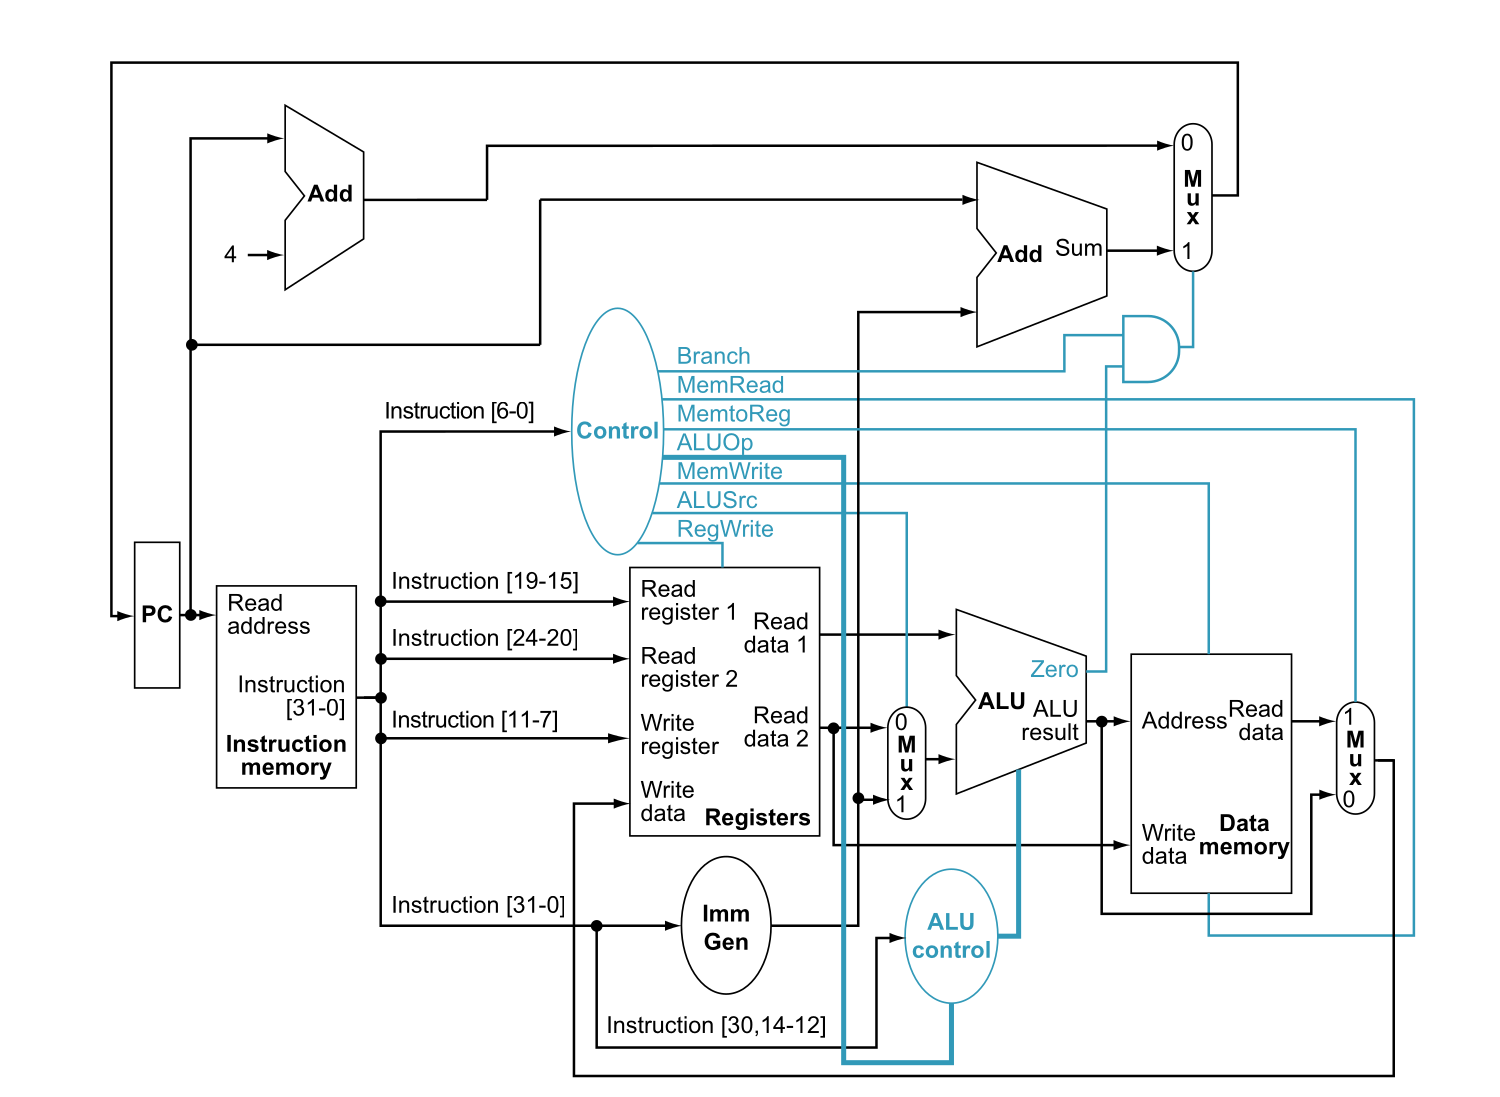
\includegraphics[width=\textwidth]{hannersy-patterson-implementation-fig4-21.png}
\fonte[Source]{Figure 4.21 of \citeonline{patterson2020} --- David A. Patterson
  and John L. Hennessy, \emph{Computer Organization and Design: RISC-V
  Edition}, 2nd ed., Morgan Kaufmann (an imprint of Elsevier), 2020.
  Reproduced here for academic purposes; copyright in the original
  illustration remains with the authors and the publisher.}
\nota[Note]{Black lines carry values and blue lines carry control signals.
  The subset has no upper-immediate path into the register file
  (\texttt{lui}), no \mbox{PC~+~4} write-back into the register file
  (\texttt{jal}, \texttt{jalr}), no register~$\rightarrow$~PC path
  (\texttt{jalr}) and no path from the \mbox{PC~+~immediate} adder into the
  register file, which only steers the PC multiplexer (\texttt{auipc}); each
  of those absences is the hardware reason for a synthesis derived in
  Section~\ref{sec:sc1-synthesis}.}
\end{figure}
